\documentclass[tikz,border=2pt]{standalone}

\usepackage{pgfplots}
\pgfplotsset{compat=1.18}
\usepgfplotslibrary{fillbetween,groupplots}

\begin{document}
	
	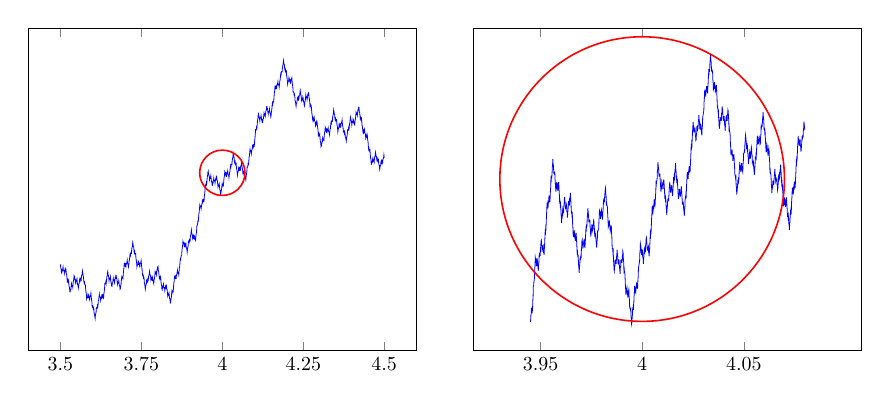
\begin{tikzpicture}[scale=0.72,
		declare function={
			weierstrass(\x) = 
			0.5*cos(deg(\x)) +
			0.25*cos(deg(3*\x)) +
			0.125*cos(deg(9*\x)) +
			0.0625*cos(deg(27*\x)) + 
			0.03125*cos(deg(81*\x)) + 
			0.015625*cos(deg(243*\x)) + 
			0.0078125*cos(deg(729*\x)) + 
			0.00390625*cos(deg(2187*\x)) + 
			0.001953125*cos(deg(6561*\x)) + 
			0.0009765625*cos(deg(19683*\x));
		}
		]
		
		\begin{groupplot}[
			group style={
				group size=2 by 1,
				horizontal sep=1cm,
			},
			samples=1000, % Increase the number of samples for better accuracy
			enlargelimits=true,
			ytick=\empty,
			axis equal,
			]
			
			% Left plot: Extended domain to [3.5, 4.5]
			\nextgroupplot[domain=3.5:4.5,
			xtick={3.5, 3.75, 4, 4.25, 4.5},
			xticklabels={$3.5$, $3.75$, $4$, $4.25$, $4.5$}
			]
			\addplot+[mark=none] {weierstrass(x)};
			\draw[red, thick] (axis cs:4,-0.1) circle [radius=0.07];
			
			% Right plot: Extended domain to [3.95, 4.05]
			\nextgroupplot[domain=3.945:4.08, 
			ytick=\empty,
			xtick={3.95, 4, 4.05}, xticklabels={$3.95$, $4$, $4.05$}]
			\addplot+[mark=none] {weierstrass(x)};
			\draw[red, thick] (axis cs:4,-0.1) circle [radius=0.07];
		\end{groupplot}
		
	\end{tikzpicture}
	
	
\end{document}